\chapter{Stand der Technik}

Bei der Simulation des Inselnetzes liegt der Fokus hinsichtlich des Stands der Technik insbesondere auf zwei Gebieten. Zum einen handelt es sich um Inselnetze als Ganzes. Dabei werden verschiedene Fragen beantwortet, u.a. welche Inselnetze in der Realität existieren oder existierten und warum dies so ist. Zum anderen werden potentielle Speicherarten betrachtet und auf das zu simulierende Inselnetz bezogen analysiert. Ziel ist es, eine technisch und wirtschaftlich realistische Betrachtung zu ermöglichen.

\section{Inselnetze}

Als Inselnetz, auch autonomes Netz genannt, wird ein Stromnetz bezeichnet, welches nur ein kleines Gebiet versorgt und keinen Anschluss an andere Stromnetze besitzt. 
Es stellt das Gegenstück zum Verbundnetz dar, welches aus mehreren kleinen, synchronisierten Netzen besteht\cite{energielexikon}. 
Es gibt verschiedene Gründe, ein Inselnetz aufzubauen. Häufige Anlässe, ein Inselnetz aufzubauen, bestehen in der geographischen isolierten Position
oder politischen Lagen von Gebieten, für die eine Stromversorgung aufrechterhalten werden soll. 
Historische Beispiele hierfür sind die Nordseeinsel Helgoland, welche bis 2009 durch Dieselgeneratoren Strom ihre Stromversorgung sicherstellte\cite{merkur} und West-Berlin, 
dessen externe Stromversorgung durch die Blockade der sowjetischen Besatzungszone 1948 binnen vier Tagen vollständig gekappt wurde\cite{berlinstreet}. 
Auch heutzutage gibt es noch Inselnetze, beispielsweise das der 30.000-Einwohner Stadt Fairbanks im US-Bundesstaat Alaska\cite{iseralaska} oder 
der Färöer-Inseln\cite{cigre-article}. 
Letzteres ist für den Aufbau des Netzes der fiktiven Kommune von größter Relevanz, da dieses momentan entwickelt wird, 
um eine Stromversorgung mit ausschließlich erneuerbaren Energien zu ermöglichen\cite{trondheim-thesis}. 
Dabei ist das Ziel Wind als primäre Energiequelle zu nutzen, was auch für das vorliegende Projekt zutrifft. Bei einer Einwohnerzahl von 54.000\cite{statista-population} und dazugehöriger Industrie und Infrastruktur liegt ein höherer Strombedarf als für dieses Projekt vor, jedoch bewegt dieser sich voraussichtlich in einer ähnlichen Größenordnung, sodass der Aufbau, untersuchte Parameter und tiefere Analysen für das fiktive Projekt relevant sind.
Weitere Inselnetze werden für beispielsweise für Flugzeuge, Schiffe oder sensible Infrastruktur, wie Krankenhäuser oder militärische Einrichtungen, betrieben. 
Diese werden nicht weiter betrachtet.
Ein Inselnetz einer Kommune kann vom Aufbau generell leicht skizziert werden. 
Es besteht im vorliegenden Fall aus einem Verteilverbund  aus Stromerzeugern und -verbrauchern, als auch Speichersystemen. 
Das Netz wird durch verschiedene technische Geräte, beispielsweise Trafos, und einer Regelung gestützt. 

\begin{figure}[h!]
    \centering
    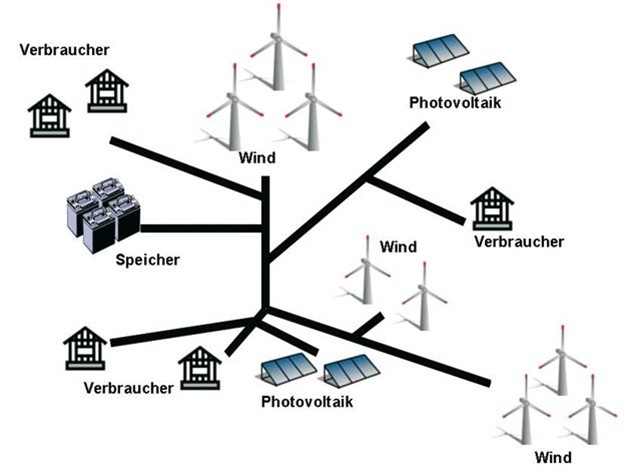
\includegraphics[width=14cm]{Abbildungen/StandDerTechnikAbb1.jpg}
    \caption{Skizze Inselnetz}\label{fig:Skizze_Inselnetz}
\end{figure}

Zu den regenerativen Stromerzeugern, welche genutzt werden können, zählen Windkraft, wobei zwischen On- und Off-Shore unterschieden wird, 
Photovoltaik, Wasserkraft und Geothermie. Die Auswahl der Stromerzeuger nach den lokalen Gegebenheiten. 
Auf den Färöer-Inseln bietet sich aufgrund der Lage insbesondere Windkraft , sowohl On-Shore als auch Off-Shore, an. 
Darüber hinaus wurde die Nutzung von Wasserkraft in Form von Gezeitenkraftwerken geprüft\cite{trondheim-thesis}. 
Auch Geothermie und Photovoltaik spielen eine Rolle. Für deutsche Kommunen sind diese Stromerzeuger auch relevant, wobei sich 
geothermische Kraftwerke ausschließlich in Süddeutschland finden lassen. 
Die Stromverbraucher setzen sich auf kommunaler Ebene aus einer Mischung aus Wohn- und Nichtwohngebäuden als auch gegebenenfalls industrieller Abnehmer zusammen. 
Als Speichersysteme kommen z. B. Batterien in Frage. In der Praxis werden häufig Lithium-Ionen oder Redox-Flow-Batterien genutzt. 
Solche Speicher, insbesondere auf Gebäudeebene, können diese zu sogenannten Prosumern  machen und schon heute ein relevanter Faktor bei der Netzregelung sein. 
Darüber hinaus fallen Wärme-, Druckluftspeicher, Pumpspeicherwerke und die Zwischenlagerung als Wasserstoff unter nutzbare Speichersysteme bei Nutzung erneuerbarer Energien. 
Zur kurzzeitigen Speicherung von Strom zur Netzstabilität ist außerdem die Nutzung von Spulen, Kondensatoren oder Schwungmassenspeichern möglich. 
Inselnetze haben im Vergleich zu Verbundnetzen eine Reihe von Vor- und Nachteilen. 
Sie können autonom operieren und unterliegen einer lokalen Kontrolle. 
Dadurch wird die Anpassung der Energieproduktion und -verteilung an die Bedürfnisse der Verbraucher einfacher. 
Außerdem sind Transportverluste und die Komplexität des Systems deutlich geringer als bei Verbundnetzen. 
Dagegen steigen die Stromerzeugungskosten, was die Wirtschaftlichkeit des Inselnetzes erschwert. 
Ein weiterer Nachteil ist, dass eine Kommune oder Inselgruppe über geographisch begrenzte Ressourcen verfügt. 
Erneuerbare Energien, beispielsweise Photovoltaik und Windkraft, sind limitiert einsetzbar und volatil gegenüber Wetterschwankungen. 
Bei anhaltender Dunkelflaute oder einer Beschädigung des Inselnetzes ist die Versorgungssicherheit eines Solchen, wie dem der Färöer-Inseln, unmittelbar gefährdet.
Insgesamt sind solche Inselnetze meist darauf ausgelegt, einen Überschuss an elektrischer Energie zu produzieren. 
Für das Stromnetz der Färöer-Inseln wurde 2021 berechnet, dass für die Tagesproduktion an Strom Kapazitäten von 224% für Wind, 105 % für PV mit 8-9 Tage Speicherkapazität gerechnet werden müssen, um eine Versorgung von 87 % aus erneuerbaren Energien zu gewährleisten\cite{researchgate-paper}.  
 
\begin{figure}[h!]
    \centering
    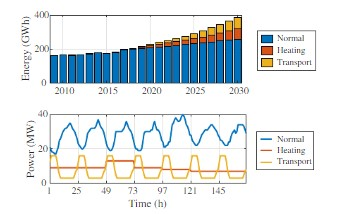
\includegraphics[width=14cm]{Abbildungen/StandDerTechnikAbb2.jpg}
    \caption{Stromprognose und Lastverläufe Färöer-Inseln, Stand 2021}\label{fig:Stromprognose_und_Lastverläufe}
\end{figure}

In solchen Prognosen ist es außerdem wichtig, Prognosen des Strombedarfs für mehrere Jahre in die Zukunft zu berücksichtigen (s. Abbildung 2). 
Die Lastverläufe sind außerdem in Kombination mit fluktuierender Stromerzeugung von hoher Relevanz für Regelung und Speicher. 
Dabei ist eine wochenbezogene Betrachtung üblich.

\section{Speicher}

Die Speicherung von Strom spielt in der Simulation eine zentrale Rolle. 
Um den Aufbau von realistischen Speichersystemen im fiktiven Inselnetz zu ermöglichen, 
ist ein Blick auf den Stand der Technik solcher Speichertechnologie notwendig. 
Im Fokus stehen dabei Be- und Entladeverhalten von genutzten Batterien, da deren Verhalten fundamental für Be- und Entladestrategien ist. 
Außerdem werden weitere Speichertechnologien genauer betrachtet, um den Nutzen ihres Einsatzes in der Simulation abzuschätzen. 
Eine Gegenüberstellung dieser Technologien nach heutigem Stand von Ausspeicherdauer zu Speicherkapazität in 
logarithmischer Skalierung kann nachfolgender Abbildung entnommen werden.

\begin{figure}[h!]
    \centering
    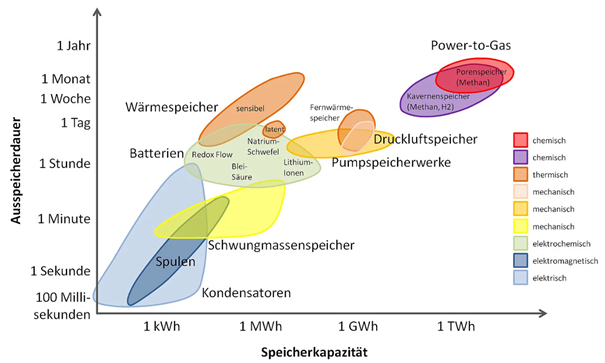
\includegraphics[width=14cm]{Abbildungen/StandDerTechnikAbb3.png}
    \caption{Speichertechnologien Übersicht}\label{fig:Speichertechnologien_Übersicht}
\end{figure}
 
Batteriespeicher gehören zu den am häufigsten genutzten Speicherformen für Inselnetze. 
Eine genauere Betrachtung der verschiedenen Batterietypen nach ihrem Stand der Technik bietet sich an. 
Relevant sind dabei insbesondere der Wirkungsgrad, die Lebens- bzw. Zyklenlebensdauer, 
der Temperaturbereich in welchem die Batterien arbeiten können und die Kosten.

%\begin{table}[htbp]
%    \centering
%    \caption{Gegenüberstellung Batteriespeicher Stand der Technik}
%    \begin{tabular}{lcccccc}
%    \label{tab:Gegenüberstellung_Batteriespeicher_Stand_der_Technik}
%        \toprule
%        \textbf{Batterietyp} & \textbf{Energiedichte [Wh/kg]} & \textbf{Wirkungsgrad [\%]} & \textbf{Lebensdauer [Jahre]} & \textbf{Zyklenlebensdauer [-]} & \textbf{Temperaturbereich [°C]} & \textbf{Kosten [€/kWh]} \\
%        \midrule
%        Blei-Säure & 25-40 & 80-90 & 3-12 & 50-2.000 & -20 bis +50 & 100-300 \\
%        Lithium-Ionen & 70-260 & 90-95 & Bis zu 15 & >2.000 & 0 bis +40 & 92 \\
%        Natrium-Ionen & 140-160 & 90 & k.A. & >50.000 & -20 bis +45 & 60\cite{energieexperten} \\
%        Nickel-Metallhybrid & 80 & 70-90 & Bis zu 10 & 500 (i.L.) & Über 0°C & 150 – 300* \\
%        Natrium-Schwefel & 218 & 75-85 & Ca. 10 & 2.500 (i.L.) & +300 bis +350 & 200 – 400* \\
%        Redox-Flow (Vanadium) & 10-85 & 70-80 & >15 & >15.000 & 0 bis +40 & 200 – 500* \\
%        \bottomrule
%    \end{tabular}
%\end{table}
%*grobe Schätzung

Unter Betrachtung der verglichenen Eigenschaften von genutzter Batteriespeicher die meisten betrachteten Technologien 
aus der Auswahl für ein Inselnetz heraus. Blei-Säure-Batterien sind für die benötigte Speicherkapazität unwirtschaftlich. 
Nickel-Metallhybrid-Batterien sind über alle Eigenschaften hinweg Lithium-Ionen-Batterien unterlegen und werden durch ebendiese momentan ersetzt. 
Da Natrium-Ionen-Batterien eine deutlich geringere Energiedichte haben, eignen sie sich 
als stationäre Batterie-Speicherkraftwerke nicht für Wind- und Solarenergie nicht. 
Bei Natrium-Schwefel-Batterien liegt bei der vorliegenden Anwendung das Hauptproblem im nutzbaren Temperaturfenster. 
Die hohen Temperaturen von 300 bis 350°C müssen gehalten werden, wodurch sie als Speicher bisher nur 
für Großspeicher zur Netzstabilisierung Anwendung gefunden haben. 
Als realisierbare Speicher bleiben Lithium-Ionen- und Redox-Flow-Batterien übrig. 
Eine tiefere Analyse folgt.

\subsection{Lithium-Ionen-Batterien}

Bei Lithium-Ionen-Batterien handelt es sich um die am häufigsten genutzte Art von Batteriespeichern. 
Dabei können diese sowohl als kleine stationäre Speicher mit einstelliger kWh-Kapazität in Prosumern, 
beispielsweise Haushalten mit PV-Anlage, oder als Großspeicher im Kapazitätsbereich von mehreren MWh genutzt werden.
Lithium-Ionen-Batterien erreichen mit bis zu 95 \% den höchsten Wirkungsgrad unter allen serienmäßigen Speicherarten. 
Darüber hinaus haben sie mit bis zu 260 Wh/kg auch die höchste Energiedichte. Die Lebensdauer von bis zu 15 Jahren 
und bis zu über 2.000 Zyklen ist vergleichsweise durchschnittlich. 
Das Operationsfenster von 0 bis 40°C ist befindet sich über den Großteil des Jahres im Rahmen der Außentemperaturen 
in Deutschland. Die Selbstentladung pro Monat bei 20°C liegt bei etwa 4 \%\cite{uni-lecture}.
Risiken bei Lithium-Ionen-Batterien liegen bei Fehlfunktionen der Lade-/Entladeelektronik oder durch Überhitzung. 
Resultierend können Feuer entstehen, deren Löschung mit herkömmlichem Löschmittel für die Feuerwehr schwierig ist.
Anwendungsbeispiele für Lithium-Ionen-Batterien als Großspeicher sind 6 und 18 MWh auf Jeju Island, 
Südkorea oder in der Automobilindustrie die Tesla-Batterie. Der Marktanteil liegt von Lithium-Ionen-Batterien liegt bei über 95\%.
Perspektivisch könnten Lithium-Ionen-Batterien von Natrium-Ionen-Batterien abgelöst werden. 
Diese sind aber bisher defizitär hinsichtlich ihrer Energiedichte, jedoch prinzipiell günstiger und thermisch robuster. 

\subsection{Redox-Flow-Batterien}

Der Aufbau einer Redox-Flow-Batterie besteht aus mindestens zwei Halbzellen. Dies ermöglicht verschiedene Materialpaarungen. 
Mögliche Materialpaarungen sind u. a. Vanadium/Vanadium, Chrom/Eisen oder Zink/Bromid. 
Da die Auswahl der Materialpaarung einen wesentlichen Einfluss auf die Energiedichte hat, 
hat sich als meistverbreitete Technologie Vanadium/Vanadium durchgesetzt. 
Der Wirkungsgrad von Redox-Flow-Batterien liegt bei 80 \%, wird jedoch durch Verluste beim Pumpvorgang des 
Elektrolyts mit 70 bis 75\% erhöht. 
Bei einer Energiedichte von bis zu 85 Wh/kg bei einer Vanadium/Vanadium-Materialpaarung liegt diese deutlich 
unter den Lithium-Ionen-Batterien. Die Lebensdauer einer Batterie kann 15 Jahre und 15.000 Zyklen überschreiten. 
Das Operationsfenster liegt bei 0 bis 40°C und entspricht dem der Lithium-Ionen-Batterie\cite{uni-lecture}. 
Die Selbstentladung pro Monat bei 20°C liegt bei unter 1 \% und ist damit marginal.
Neben der geringeren Energiedichte der Batterien, welche mit einem größeren Platzbedarf im stationären Betrieb eingehen, 
haben Redox-Flow-Batterien einen Faktor der finanziellen Ungewissheit in der Herstellung. 
Dies liegt daran, dass die effizienteste Materialpaarung aus Vanadium besteht, welches als kritischer Rohstoff gilt und 
starken Preisschwankungen unterliegt\cite{cleanthinking}.
Die Technologie der Redox-Flow-Batterien ist weniger gut erforscht als die der Lithium-Ionen-Batterien und wird aktuell stärker erforscht, 
da größeres Potential für Verbesserungen vermutet wird. 
Bereits 2020 wurde an der University of South California eine Anthrachinondisulfonsäure/Eisensulfat-Materialpaarung genutzt, 
mit der Kosten von 54 €/kWh\cite{yang2020redoxflow} erzielt werden konnten. Damit liegt man im Kostenbereich von Natrium-Ionen-Batterien und 
unter Lithium-Ionen-Batterien. Langfristig ist eine kommerzielle Nutzung von Redox-Flow-Batterien als Großspeicher denkbar. 
Ein Pionierprojekt in der Wirtschaft stellt der Bau eines 500 MWh-Redox-Flow-Speichers der LEAG in Boxberg dar. 
Bei diesem Projekt handelt es sich bisher allerdings nur um eine Planung, die bis 2027 umgesetzt werden soll\cite{winfuture-news}.

\subsection{Aufbau von stationären Batteriespeichersystemen}

In einem kommunalen Inselnetz werden häufig ein oder mehrere stationäre Batteriespeichersysteme genutzt. 
In dem hier betrachteten Kapazitätsbereich von mehreren MW spricht man von Großspeichern. 
Im Zuge der Energiewende haben sich Schwerpunkte des Anforderungsprofils solcher Batteriegroßspeicher verändert. 
Wichtige Eigenschaften stellen dabei die Reaktionsgeschwindigkeit, Flexibilität und Zuverlässigkeit solcher Systeme dar.
 
\begin{figure}[h!]
    \centering
    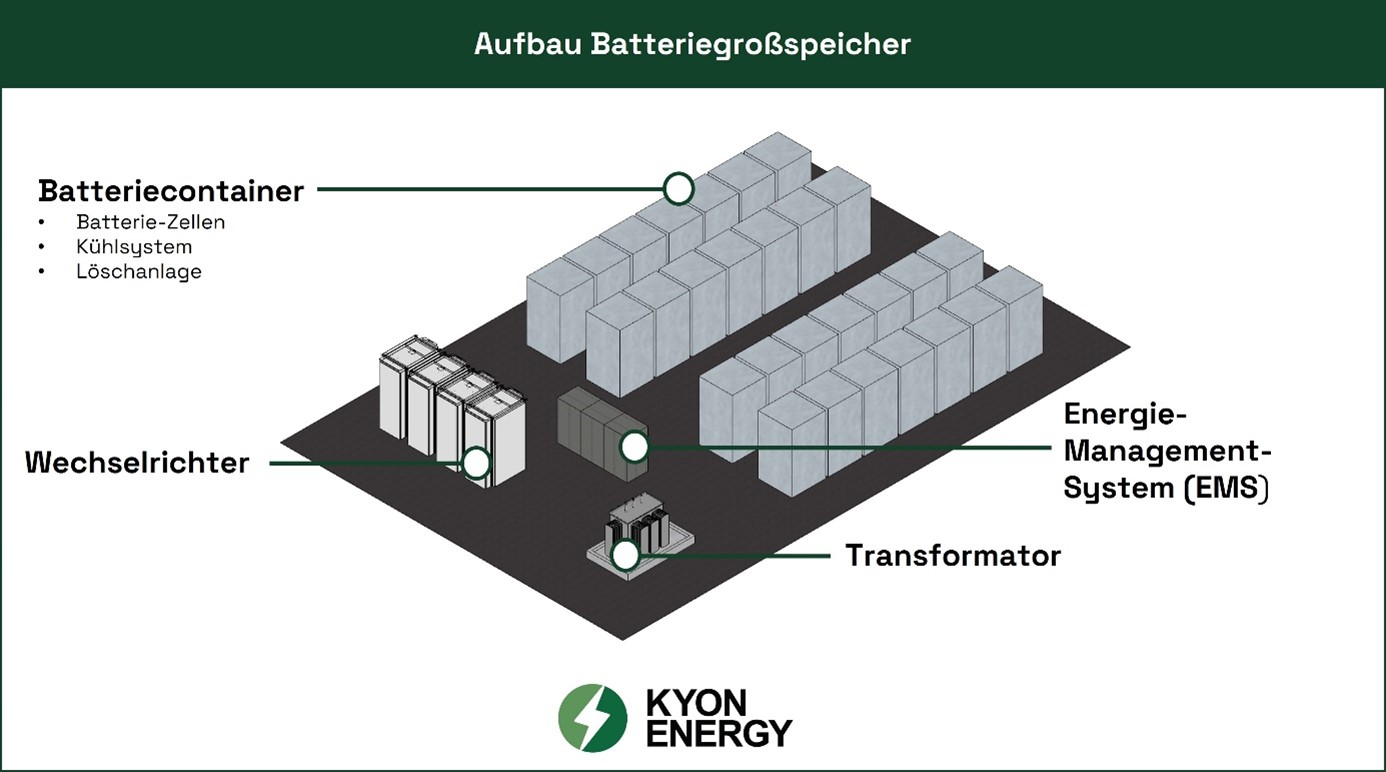
\includegraphics[width=14cm]{Abbildungen/StandDerTechnikAbb4jpg.jpg}
    \caption{Batterispeichersystem Aufbau}\label{fig:Batterispeichersystem_Aufbau}
\end{figure}

Ausgangspunkt des Speichers sind die Batteriezellen in einem Container. 
Um die technischen und gesetzlichen Anforderungen zu erfüllen, besitzt jeder Batteriecontainer ein Kühlsystem für die Nutzung und eine Löschanlage für den Brandfall. 
Diese Batteriecontainer können flexibel skaliert werden, also an die Bedürfnisse des Stromnetzes angepasst werden. 
Im Vergleich zu anderen Industrieren wie z.B. der Automobilindustrie, spielt die Energiedichte eine geringere Rolle, als reine Materialkosten. 
Daher werden häufig billigere Zellen aus Lithium-Eisen-Phosphat (LFP), der Alternative mit hoher Energiedichte aus Lithium-Nickel-Mangan-Cobalt (NMC), vorgezogen.

\begin{table}[htbp]
    \centering
    \caption{Auswahl Batteriezellen Großspeicher\cite{poworks-comparison}}
    \label{tab:Auswahl_Batteriezellen_Großspeicher}
    \begin{tabular}{lcccc}
       \toprule
        & \textbf{LFP} & \textbf{NMC} & \textbf{Redox Flow} & \textbf{Redox Flow (Vanadium-Vanadium)} \\
        \midrule
        \textbf{Energiedichte [Wh/kg]} & 230-260 & 130-200 & 10-85 & 85 \\
        \textbf{Kosten [€/kWh]} & 150-250 & 100-200 & 200-500* & 300-500* \\
        \bottomrule
    \end{tabular}
\end{table}

* grobe Schätzung

Da Batterien im Gleichstrom betrieben werden, wird das Batteriesystem durch Wechselrichter vom Netz getrennt. 
Wenn die vorliegenden Energiemengen entsprecht groß sind, bedarf es außerdem eines Transformators, w
elcher den Strom von der Niederspannungsebene auf das gewünschte Spannungsniveau wandelt. 
Wechselrichter und Transformatoren müssen bidirektional verwendbar sein, um Be- und Entladung zu gewähren. 
Die Koordination dieses Vorganges wird durch ein Energie-Management-System (EMS) gewährleistet. 
Dadurch ist es außerdem möglich, Zellen zu überwachen und das System im Problemfall zu schützen\cite{kyon-energy}.

